% IEEE Conference Template for ML/AI Papers
% Document class specification - conference format for IEEE
\documentclass[conference]{IEEEtran}

% Override command lockouts (typically needed for IEEE papers)
\IEEEoverridecommandlockouts
% The preceding line is only needed to identify funding in the first footnote. If that is unneeded, please comment it out.

%%%%%%%%%%%%%%%%%%%%%%%%%%%%%%%%%%%%%%%%%
% PACKAGES
%%%%%%%%%%%%%%%%%%%%%%%%%%%%%%%%%%%%%%%%%
% Citation management
\usepackage{cite}                    % For bibliography citations

% Text and list formatting
\usepackage{enumitem}                % Enhanced list environments
\usepackage{amsmath,amssymb,amsfonts} % Mathematical symbols and fonts

% Algorithms
\usepackage{algorithm}               % For algorithm environments
\usepackage{algorithmic}             % For algorithm formatting

% Graphics and visual elements
\usepackage{graphicx}                % For including images
\usepackage{textcomp}                % Text companion fonts
\usepackage{xcolor}                  % For colored text
\usepackage{forest}                  % For drawing tree diagrams

% TikZ and related packages for diagrams
\usepackage{tikz}                    % Core package for creating graphics
\usepackage{adjustbox}               % For scaling figures
\usepackage{url}                     % For formatting URLs

% Figure and table enhancements
\usepackage{pgfplots}                % For creating plots
\usepackage{booktabs}                % For professional-looking tables
\usepackage{colortbl}                % For colored table cells
\pgfplotsset{compat=1.18}

% TikZ libraries for specific diagram types
\usetikzlibrary{shapes.geometric,arrows,positioning,fit,backgrounds,calc,decorations.pathreplacing,decorations.markings,patterns,circuits.logic.US,matrix,chains}

% Table enhancements
\usepackage{threeparttable}          % For table notes
\usepackage{cuted}                   % For multi-column environments

% Custom command for line breaks in author block
\makeatletter
\newcommand{\linebreakand}{%
  \end{@IEEEauthorhalign}
  \hfill\mbox{}\par
  \mbox{}\hfill\begin{@IEEEauthorhalign}
}
\makeatother

% Define custom colors for visualizations
% These are common colors used in AI/ML papers
\definecolor{qubitblue}{RGB}{70,130,180}      % Blue for primary elements
\definecolor{controlred}{RGB}{220,20,60}      % Red for control elements
\definecolor{aigreen}{RGB}{50,150,50}         % Green for AI components
\definecolor{quantumpurple}{RGB}{128,0,128}   % Purple for quantum elements
\definecolor{errororange}{RGB}{255,140,0}     % Orange for error highlighting

%%%%%%%%%%%%%%%%%%%%%%%%%%%%%%%%%%%%%%%%%
% DOCUMENT BEGINS
%%%%%%%%%%%%%%%%%%%%%%%%%%%%%%%%%%%%%%%%%
\begin{document}
\raggedbottom

%%%%%%%%%%%%%%%%%%%%%%%%%%%%%%%%%%%%%%%%%
% TITLE SECTION
%%%%%%%%%%%%%%%%%%%%%%%%%%%%%%%%%%%%%%%%%
\title{Modern Text-to-Image Generation (2020--2025): Diffusion Transformers, Token Models, and Controllable Synthesis}

\author{
    \IEEEauthorblockN{Author Name(s) TBD}
    \IEEEauthorblockA{Affiliation(s) TBD\\Email(s) TBD}
}

\maketitle

%%%%%%%%%%%%%%%%%%%%%%%%%%%%%%%%%%%%%%%%%
% KEYWORDS
%%%%%%%%%%%%%%%%%%%%%%%%%%%%%%%%%%%%%%%%%
\begin{IEEEkeywords}
generative image models, text-to-image, diffusion models, diffusion transformers, autoregressive models, controllable synthesis, image editing
\end{IEEEkeywords}

%%%%%%%%%%%%%%%%%%%%%%%%%%%%%%%%%%%%%%%%%
% ABSTRACT
%%%%%%%%%%%%%%%%%%%%%%%%%%%%%%%%%%%%%%%%%
\begin{abstract}
Generative image modeling has progressed from specialized unconditional synthesis to broadly capable text-conditioned
generation and editing systems. This review surveys state-of-the-art methods from 2020--2025, with an emphasis on the two
dominant families of modern systems: diffusion/score/flow-based generators and token-based transformer models. We present a
unifying taxonomy organized around objectives, representations (pixel, continuous latent, and discrete tokens), and inference
choices (samplers/solvers, guidance, and distillation/consistency accelerations). We then synthesize architectural trends,
including the transition from U-Net backbones to diffusion transformers and scaling recipes that enable high-resolution,
photorealistic outputs. Beyond base model quality, we review mechanisms for controllability and image editing, covering
structured conditioning (e.g., geometry/layout signals), modular adapters, personalization via finetuning or embeddings, and
instruction-driven edits. We discuss evaluation protocols for conditional generation, contrasting fidelity/diversity metrics
with text--image alignment scores and highlighting failure modes that are under-captured by standard benchmarks. Finally, we
survey emerging evidence on privacy risks (memorization and training data extraction) and provenance techniques such as
watermarking, and we outline open research problems and reporting practices needed for reproducible and responsible progress.
\end{abstract}

%%%%%%%%%%%%%%%%%%%%%%%%%%%%%%%%%%%%%%%%%
% INTRODUCTION
%%%%%%%%%%%%%%%%%%%%%%%%%%%%%%%%%%%%%%%%%
\section{Introduction and Scope}
Generative image modeling has rapidly shifted from narrow, style-specific synthesis to broadly capable
text-conditioned generation and editing systems that can be steered by prompts and auxiliary controls. The
current state of the art (SOTA) is driven by large-scale training on image--text corpora and advances in
diffusion-style objectives, guidance, and scalable backbones \cite{ho2020ddpm,ho2022cfg,rombach2022ldm,saharia2022imagen}.

This review focuses on modern text-to-image generation and image editing/inpainting, with an emphasis on
the 2020--2025 period and a cutoff date of \textbf{2025-12-27}. We treat SOTA as a multi-objective frontier
that balances fidelity, diversity, prompt adherence, controllability, and inference cost, rather than a single metric
leaderboard \cite{heusel2017fid,hessel2021clipscore}. We also highlight that ``frontier'' systems often differ in
what they disclose (data, compute, training details), which directly affects reproducibility and scientific interpretability
\cite{schuhmann2022laion5b,rombach2022ldm}.

Our angle is pragmatic: we organize the space around (i) \emph{model families} (diffusion/score/flow, token-based
autoregressive or masked modeling, and high-fidelity GANs), (ii) \emph{conditioning and control} mechanisms for
steerable synthesis and editing, and (iii) \emph{evaluation and failure modes} that matter in real deployments
\cite{chang2022maskgit,peebles2022dit,zhang2023controlnet}. Throughout, we prioritize primary sources for each method
and explicitly separate evidence-backed claims from common but weakly supported folklore.

The remainder of the paper is structured as follows: Section~II introduces core objectives, representations, and
inference choices; Sections~III--V cover diffusion models, token-based generators, and controllable/editable generation;
Section~VI surveys frontier systems and practical tradeoffs; Sections~VII--VIII discuss evaluation, safety, provenance,
and open problems \cite{song2020ddim,lu2022dpmsolver,brooks2022instructpix2pix}.

%%%%%%%%%%%%%%%%%%%%%%%%%%%%%%%%%%%%%%%%%
% BACKGROUND
%%%%%%%%%%%%%%%%%%%%%%%%%%%%%%%%%%%%%%%%%
\section{Foundations and Building Blocks}
\subsection{Objectives and Formulations (Minimal Math)}
Modern generative image models can be grouped by their training objective and sampling procedure. Diffusion
models learn to reverse a forward noising process and typically sample by iterative denoising
\cite{ho2020ddpm,song2020ddim}. Score-based formulations connect diffusion to stochastic differential equations,
which clarifies sampler design and continuous-time perspectives \cite{song2021sdescore}. In practice, a key unifying
axis is \emph{conditioning}: most SOTA systems are conditional generators where text, images, and/or structured controls
define the output distribution \cite{rombach2022ldm,saharia2022imagen}.

Token-based approaches instead reduce image generation to sequence modeling over discrete codes, using either
autoregressive factorization or masked token prediction \cite{oord2017vqvae,esser2020vqgan,chang2022maskgit}. While
GANs remain competitive for specific domains and high-fidelity unconditional synthesis, recent SOTA for text-to-image
is dominated by diffusion and token-based families \cite{karras2019stylegan2,kang2023gigagan}.

Figure~\ref{fig:taxonomy} provides a high-level taxonomy of these families that we use throughout the review.

\begin{figure}[t]
    \centering
    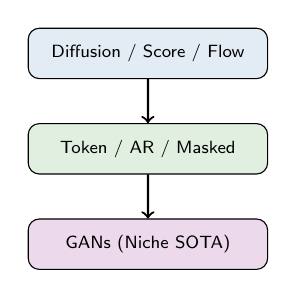
\begin{tikzpicture}[
        scale=0.8, transform shape,
        node distance=0.7cm,
        % Prefer low-saturation fills for readability in two-column papers.
        box/.style={rectangle, rounded corners, draw, fill=#1!15, text=black,
            minimum width=3.8cm,
            minimum height=0.8cm,
            align=center, font=\sffamily\footnotesize}
    ]
        \node[box=qubitblue] (node1) {Diffusion / Score / Flow};
        \node[box=aigreen, below=of node1] (node2) {Token / AR / Masked};
        \node[box=quantumpurple, below=of node2] (node3) {GANs (Niche SOTA)};

        % Connections
        \draw[->, thick] (node1) -- (node2);
        \draw[->, thick] (node2) -- (node3);
    \end{tikzpicture}
    \caption{Taxonomy of modern generative image model families (diffusion/score/flow; token-based AR/masked; and GANs), grounded in representative works such as DDPMs \cite{ho2020ddpm}, DiTs \cite{peebles2022dit}, masked token generators \cite{chang2022maskgit}, and StyleGAN-style GANs \cite{karras2019stylegan2}.}
    \label{fig:taxonomy}
\end{figure}

\subsection{Conditioning, Guidance, and Encoders}
Text conditioning is typically implemented by encoding prompts into embeddings that modulate a generative backbone
via cross-attention or related mechanisms \cite{radford2021clip,rombach2022ldm}. Beyond conditioning, \emph{guidance}
methods modify the sampling trajectory to trade off sample quality and prompt adherence. Classifier-free guidance (CFG)
has become a default choice because it avoids training an external classifier while providing a strong quality--alignment
knob \cite{ho2022cfg}. These mechanisms interact with model class: diffusion samplers and token decoders expose different
control surfaces and failure modes, motivating careful comparisons across families \cite{song2020ddim,chang2023muse}.

\subsection{Backbones and Representations}
Representation choices strongly shape compute and controllability. Latent diffusion models generate in a learned latent
space rather than pixel space, enabling high-resolution synthesis at reduced cost while keeping a diffusion-style training
objective \cite{rombach2022ldm}. In parallel, diffusion transformers (DiTs) replace U-Net backbones with transformer
architectures that scale well and unify image generation with broader transformer design patterns \cite{peebles2022dit,chen2023pixartalpha}.

Token-based generators rely on discrete tokenizers (e.g., VQ-style codebooks) that compress images into sequences of codes,
so generation becomes token prediction \cite{oord2017vqvae,esser2020vqgan}. This design can support fast decoding and
scaling regimes closer to language modeling, but also introduces tokenization artifacts and additional reconstruction loss
that can limit fine detail \cite{chen2020imagegpt,chang2022maskgit}.

\subsection{Sampling, Solvers, and Efficiency}
Inference cost is often dominated by the number of sampling steps and backbone evaluations. For diffusion, deterministic
or ODE-inspired samplers reduce the number of steps required for high-quality outputs \cite{song2020ddim,lu2022dpmsolver}.
The design space of noise schedules and parameterizations further impacts sampling efficiency and robustness
\cite{karras2022edm}. Distillation and consistency-style training aims to compress long denoising chains into few-step
generators, enabling real-time or interactive use cases \cite{salimans2022progressivedistill,song2023consistency,luo2023lcm}.

%%%%%%%%%%%%%%%%%%%%%%%%%%%%%%%%%%%%%%%%%
% BUILDING BLOCKS / TAXONOMY
%%%%%%%%%%%%%%%%%%%%%%%%%%%%%%%%%%%%%%%%%
\section{Diffusion Models: From DDPMs to Diffusion Transformers}
\subsection{Training Objectives and Noise/SDE/Flow Views}
Diffusion probabilistic models define a forward noising process that gradually perturbs data $x_0$ into $x_t$,
and learn a reverse-time model to denoise from noise back to samples \cite{ho2020ddpm}. A common parameterization
trains a network to predict the injected noise $\epsilon$ under a mean-squared error objective:
\begin{equation}
\begin{aligned}
    \mathcal{L}_{\mathrm{simple}}(\theta)
    &=
    \mathbb{E}_{t, x_0, \epsilon}\left[
        \lVert \epsilon - \epsilon_\theta(x_t, t, c) \rVert_2^2
    \right], \\
    x_t &= \sqrt{\bar{\alpha}_t} x_0 + \sqrt{1-\bar{\alpha}_t}\,\epsilon.
\end{aligned}
\end{equation}
where $c$ denotes conditioning (e.g., text embeddings) \cite{ho2020ddpm,rombach2022ldm}.

Score-based generative modeling frames the reverse process via the score function $\nabla_{x_t} \log p_t(x_t)$ and
connects diffusion to SDEs, which provides a principled way to derive samplers and understand continuous-time limits
\cite{song2021sdescore}. Recent ``flow'' and ``rectified flow'' perspectives further blur the boundary between diffusion-like
training and ODE-style generation, and have been combined with transformer backbones for high-resolution synthesis
\cite{esser2024rectifiedflow}.

\subsection{Guidance and Conditioning}
Most modern diffusion systems are conditional, and conditioning is typically injected via cross-attention, feature-wise
modulation, or related mechanisms \cite{rombach2022ldm,saharia2022imagen}. Classifier-free guidance builds a guided score
by interpolating conditional and unconditional predictions, improving prompt adherence at the cost of reduced diversity
and potential artifacts when guidance is pushed too high \cite{ho2022cfg}. In practice, guidance interacts with the
sampler/solver choice and the backbone, so comparing models without controlling these factors can be misleading
\cite{karras2022edm,lu2022dpmsolver}.

\subsection{Samplers/Solvers and Fast Sampling}
Sampling speed is a central practical bottleneck. DDIM showed that deterministic, non-Markovian sampling can produce
high-quality images with fewer steps than ancestral DDPM sampling \cite{song2020ddim}. Subsequent solver-based methods
use ODE approximations to achieve further reductions in function evaluations, often with strong empirical performance
\cite{lu2022dpmsolver}. EDM highlighted that parameterization and noise schedule choices materially affect sampling
efficiency and stability across compute budgets \cite{karras2022edm}.

Beyond better solvers, distillation and consistency training compress multi-step denoising into few-step generators.
Progressive distillation iteratively halves the number of steps while preserving a teacher's distributional behavior
\cite{salimans2022progressivedistill}. Consistency models aim to learn a mapping that is consistent across noise levels,
enabling sampling with very few steps, and latent consistency models adapt this idea to latent diffusion backbones for
efficient high-resolution synthesis \cite{song2023consistency,luo2023lcm}.

Figure~\ref{fig:diffusion-pipeline} summarizes a typical conditional diffusion sampling pipeline and highlights where guidance
and solver choices enter.

\begin{figure}[t]
    \centering
    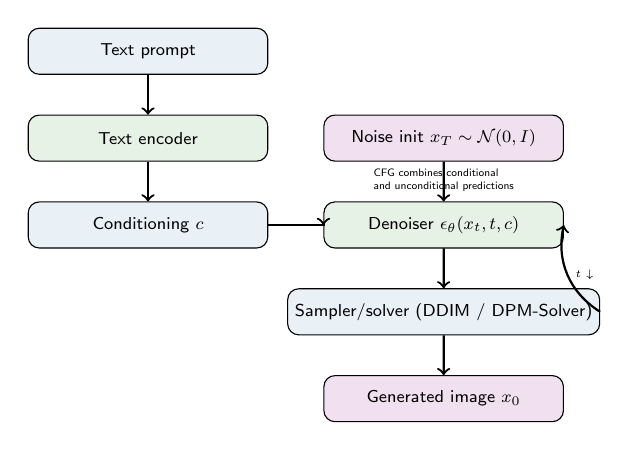
\begin{tikzpicture}[
        scale=0.78, transform shape,
        node distance=0.65cm and 0.9cm,
        box/.style={rectangle, rounded corners, draw, fill=#1!12, text=black,
            minimum width=3.9cm,
            minimum height=0.75cm,
            align=center, font=\sffamily\footnotesize}
    ]
        \node[box=qubitblue] (prompt) {Text prompt};
        \node[box=aigreen, below=of prompt] (encoder) {Text encoder};
        \node[box=qubitblue, below=of encoder] (cond) {Conditioning $c$};

        \node[box=quantumpurple, right=of encoder] (noise) {Noise init $x_T \sim \mathcal{N}(0,I)$};
        \node[box=aigreen, below=of noise] (denoiser) {Denoiser $\epsilon_\theta(x_t, t, c)$};
        \node[box=qubitblue, below=of denoiser] (solver) {Sampler/solver (DDIM / DPM-Solver)};
        \node[box=quantumpurple, below=of solver] (image) {Generated image $x_0$};

        \draw[->, thick] (prompt) -- (encoder);
        \draw[->, thick] (encoder) -- (cond);
        \draw[->, thick] (cond.east) -| (denoiser.west);
        \draw[->, thick] (noise) -- (denoiser);
        \draw[->, thick] (denoiser) -- (solver);
        \draw[->, thick] (solver) -- (image);

        \draw[->, thick, bend left=35] (solver.east) to node[right, font=\sffamily\tiny] {$t\downarrow$} (denoiser.east);
        \node[font=\sffamily\tiny, align=left] at ($(denoiser.north)+(0,0.35)$) {CFG combines conditional\\and unconditional predictions};
    \end{tikzpicture}
    \caption{Schematic diffusion sampling pipeline: start from noise and iteratively denoise with conditioning and guidance, using samplers/solvers and accelerations \cite{ho2020ddpm,ho2022cfg,song2020ddim,lu2022dpmsolver,luo2023lcm}.}
    \label{fig:diffusion-pipeline}
\end{figure}

\subsection{Architectural Evolution: Latent Diffusion, DiT, PixArt, Rectified Flow}
Architecturally, latent diffusion models popularized training diffusion in an autoencoder latent space, making
high-resolution text-to-image feasible on commodity hardware while retaining controllability via conditioning
\cite{rombach2022ldm}. Diffusion transformers (DiT) demonstrated that transformer backbones can scale diffusion models
effectively, aligning image generation with the broader trend toward transformer scalability and modularity
\cite{peebles2022dit}. More recent DiT-style systems emphasize data curation, training efficiency, and scaling recipes
for photorealistic synthesis at higher resolutions \cite{chen2023pixartalpha,chen2024pixartsigma}.

Rectified-flow transformers can be viewed as part of the same trajectory toward transformer backbones and ODE-like
generation mechanisms, aiming to improve both quality and sampling efficiency at high resolutions \cite{esser2024rectifiedflow}.

%%%%%%%%%%%%%%%%%%%%%%%%%%%%%%%%%%%%%%%%%
% TOKEN / AR MODELS
%%%%%%%%%%%%%%%%%%%%%%%%%%%%%%%%%%%%%%%%%
\section{Autoregressive and Token-Based Image Generators}
\subsection{Discrete Tokenizers and Latent Codes}
Token-based generators factor image synthesis into two stages: (i) a tokenizer that maps images into discrete code sequences,
and (ii) a sequence model that generates those codes. Vector-quantized autoencoders introduced this paradigm by learning
a discrete codebook and an encoder/decoder pair, enabling compression into a grid of tokens while maintaining visual fidelity
\cite{oord2017vqvae}. VQGAN improved perceptual quality by combining discrete latents with adversarial and perceptual losses,
making token reconstruction sharper and better aligned with human perception \cite{esser2020vqgan}.

The benefit is that generation becomes token prediction, which can exploit transformer scaling and potentially reduce sampling
steps relative to diffusion-style denoising \cite{chen2020imagegpt,yu2022parti}. The cost is that tokenizer design imposes a
rate--distortion tradeoff: aggressive compression can destroy fine detail, while high token rates increase sequence length and
compute \cite{oord2017vqvae,esser2020vqgan}.

\subsection{Autoregressive vs Masked Modeling}
Autoregressive (AR) models generate tokens sequentially, which provides a straightforward likelihood factorization but can be
latency-limited for large images \cite{chen2020imagegpt,yu2022parti}. Masked modeling instead predicts subsets of tokens in
parallel, iteratively refining a partially masked canvas. MaskGIT showed that masked generative transformers can dramatically
reduce generation time via parallel decoding while retaining strong sample quality \cite{chang2022maskgit}. Muse extended the
masked-token approach to high-quality text-to-image generation with large-scale training and guidance-like mechanisms in token
space \cite{chang2023muse}.

\subsection{Tradeoffs vs Diffusion}
Diffusion models and token-based models differ in how compute is spent. Diffusion typically requires tens of denoising steps,
but each step can be heavily optimized with solvers and distillation \cite{lu2022dpmsolver,song2023consistency,luo2023lcm}.
Token models can amortize work into a tokenizer and benefit from parallel decoding, but may be sensitive to tokenization
artifacts and can struggle to preserve high-frequency detail without long sequences or improved tokenizers \cite{esser2020vqgan,chang2022maskgit}.

In practice, SOTA systems increasingly hybridize ideas: diffusion uses transformer backbones and latent representations
\cite{rombach2022ldm,peebles2022dit}, while token models adopt guidance-like mechanisms and large-scale conditioning
\cite{chang2023muse,yu2022parti}. As a result, comparisons should report not only output quality but also throughput, latency,
and controllability under realistic constraints \cite{heusel2017fid,hessel2021clipscore}.

%%%%%%%%%%%%%%%%%%%%%%%%%%%%%%%%%%%%%%%%%
% CONTROL / EDITING
%%%%%%%%%%%%%%%%%%%%%%%%%%%%%%%%%%%%%%%%%
\section{Conditioning, Control, Personalization, and Editing}
\subsection{Conditional Inputs (Layout, Depth, Pose, Edges, Reference Images)}
Beyond text prompts, modern systems accept structured signals to constrain composition and geometry. Common conditioning
modalities include edge maps, depth, pose, segmentation, and reference images, which allow users to specify layout while
delegating texture and style to the generator \cite{zhang2023controlnet}. These controls are particularly important in
applications where spatial accuracy matters (product design, storytelling, scientific illustration), and they expose a key
gap between prompt-based benchmarks and real-world workflows \cite{brooks2022instructpix2pix}.

\subsection{Adapters and Control Networks}
Control is often implemented via lightweight modules that modulate a frozen base model. ControlNet adds a conditional branch
that injects control features into a diffusion backbone while retaining the base model's generative capability \cite{zhang2023controlnet}.
This adapter-style pattern aligns with broader trends in parameter-efficient finetuning, enabling multiple controls (e.g., pose,
depth) to share a common foundation model without retraining from scratch \cite{hu2021lora,rombach2022ldm}.

Figure~\ref{fig:control-landscape} summarizes how control, personalization, and editing modules relate to a shared base generator.

\begin{figure*}[t]
    \centering
    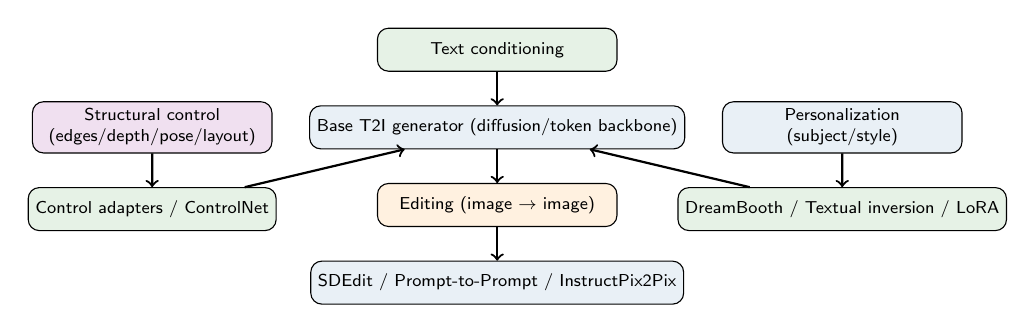
\begin{tikzpicture}[
        scale=0.78, transform shape,
        node distance=0.55cm and 0.6cm,
        box/.style={rectangle, rounded corners, draw, fill=#1!12, text=black,
            minimum width=3.9cm,
            minimum height=0.70cm,
            align=center, font=\sffamily\footnotesize}
    ]
        \node[box=qubitblue] (base) {Base T2I generator (diffusion/token backbone)};
        \node[box=aigreen, above=of base] (text) {Text conditioning};
        \draw[->, thick] (text) -- (base);

        \node[box=quantumpurple, left=of base] (control) {Structural control\\(edges/depth/pose/layout)};
        \node[box=aigreen, below=of control] (controlnet) {Control adapters / ControlNet};
        \draw[->, thick] (control) -- (controlnet);
        \draw[->, thick] (controlnet) -- (base);

        \node[box=qubitblue, right=of base] (personal) {Personalization\\(subject/style)};
        \node[box=aigreen, below=of personal] (peft) {DreamBooth / Textual inversion / LoRA};
        \draw[->, thick] (personal) -- (peft);
        \draw[->, thick] (peft) -- (base);

        \node[box=errororange, below=of base] (editing) {Editing (image $\rightarrow$ image)};
        \node[box=qubitblue, below=of editing] (methods) {SDEdit / Prompt-to-Prompt / InstructPix2Pix};
        \draw[->, thick] (base) -- (editing);
        \draw[->, thick] (editing) -- (methods);
    \end{tikzpicture}
    \caption{Control and editing landscape for modern text-to-image systems: structural controls via ControlNet-style adapters \cite{zhang2023controlnet}, personalization via finetuning/embeddings \cite{ruiz2022dreambooth,gal2022textualinversion,hu2021lora}, and editing methods \cite{meng2021sdedit,hertz2022prompttoprompt,brooks2022instructpix2pix}.}
    \label{fig:control-landscape}
\end{figure*}

\subsection{Personalization and Finetuning}
Personalization methods adapt a text-to-image model to a specific subject or style using a small number of reference images.
DreamBooth finetunes a diffusion model to bind a unique token to a subject, enabling consistent generation of that subject
in novel contexts \cite{ruiz2022dreambooth}. Textual inversion instead optimizes a new embedding vector in the text encoder
space, which can be cheaper and more modular but may be less expressive than full finetuning \cite{gal2022textualinversion}.
LoRA-style low-rank updates provide a parameter-efficient alternative that is widely used to distribute lightweight adapters
for styles, characters, and domains \cite{hu2021lora}.

These methods introduce practical risks: identity drift (loss of subject fidelity), overfitting, and potential memorization
of training images if finetuning is performed without safeguards \cite{ruiz2022dreambooth,gal2022textualinversion}. Reliable
evaluation therefore needs both qualitative inspection and quantitative probes for memorization and leakage \cite{heusel2017fid,kynkaanniemi2019pr}.

\subsection{Instruction Editing}
Editing tasks aim to modify an input image while preserving irrelevant content. SDEdit framed editing as partially noising
an input and denoising under a conditional model, enabling a range of edits without explicit supervision
\cite{meng2021sdedit}. Prompt-to-Prompt showed that manipulating cross-attention maps during diffusion sampling can yield
fine-grained, localized edits while maintaining structure \cite{hertz2022prompttoprompt}. InstructPix2Pix learns to follow
natural-language editing instructions by combining image inputs, text instructions, and diffusion-style generation
\cite{brooks2022instructpix2pix}.

More broadly, early text-guided diffusion systems demonstrated practical image editing and inpainting capabilities that
helped establish editing as a first-class use case for conditional generators \cite{nichol2021glide,ramesh2022dalle2}.

Across editing methods, common failure modes include unintended global changes (``collateral edits''), poor disentanglement
between content and style, and prompt sensitivity that reduces reproducibility \cite{hertz2022prompttoprompt,brooks2022instructpix2pix}.

%%%%%%%%%%%%%%%%%%%%%%%%%%%%%%%%%%%%%%%%%
% FRONTIER SYSTEMS
%%%%%%%%%%%%%%%%%%%%%%%%%%%%%%%%%%%%%%%%%
\section{Frontier Systems and Practical Tradeoffs (2023--2025)}
\subsection{What Counts as ``Frontier''}
We define ``frontier'' systems as those that push the Pareto boundary along at least one axis of practical capability:
photorealism, prompt adherence, controllability/editing, inference efficiency, or resolution. Importantly, frontier status is
also constrained by \emph{disclosure}: systems differ in how much they reveal about training data, compute, and implementation,
which affects how strongly we can attribute observed behavior to specific design choices \cite{rombach2022ldm,schuhmann2022laion5b}.

\subsection{Representative Systems (Open vs Closed)}
Open and reproducible research systems often publish architectures and training recipes, enabling meaningful ablation and
follow-up work. Representative examples include latent diffusion models and their descendants \cite{rombach2022ldm}, diffusion
transformers and scaled training pipelines \cite{peebles2022dit,chen2024pixartsigma}, and rectified-flow transformer variants
that target high-resolution synthesis \cite{esser2024rectifiedflow}. Token-based systems such as Parti and Muse illustrate how
large-scale token modeling can compete in text-to-image settings, albeit with different tradeoffs and disclosure patterns
\cite{yu2022parti,chang2023muse}.

Closed or partially closed systems may publish high-level technical reports without releasing weights or data, which limits
reproducibility but can still contribute valuable ideas (e.g., data curation, evaluation protocols). When discussing such
systems, we treat claims as conditional on the published evidence and avoid extrapolating beyond what is documented
\cite{saharia2022imagen,ramesh2022dalle2}.

\subsection{Efficiency and Deployment Constraints}
Deployment imposes constraints that are often invisible in academic benchmarks: latency targets, memory ceilings, and
content safety requirements. On the modeling side, fast sampling is enabled by improved solvers, distillation, and
consistency-style training \cite{lu2022dpmsolver,salimans2022progressivedistill,luo2023lcm}. On the product side,
systems frequently layer safety filters, prompt classifiers, and post-generation moderation, which can change observed
behavior relative to the underlying generator \cite{ramesh2022dalle2}.

Table~\ref{tab:frontier-models} provides an illustrative comparison of representative systems and the disclosure patterns
that affect reproducibility.

Figure~\ref{fig:timeline} provides an annotated timeline of representative research milestones that motivated key shifts in
backbones, conditioning/control, and efficiency/provenance practices across modern text-to-image systems.

\begin{figure*}[t]
    \centering
    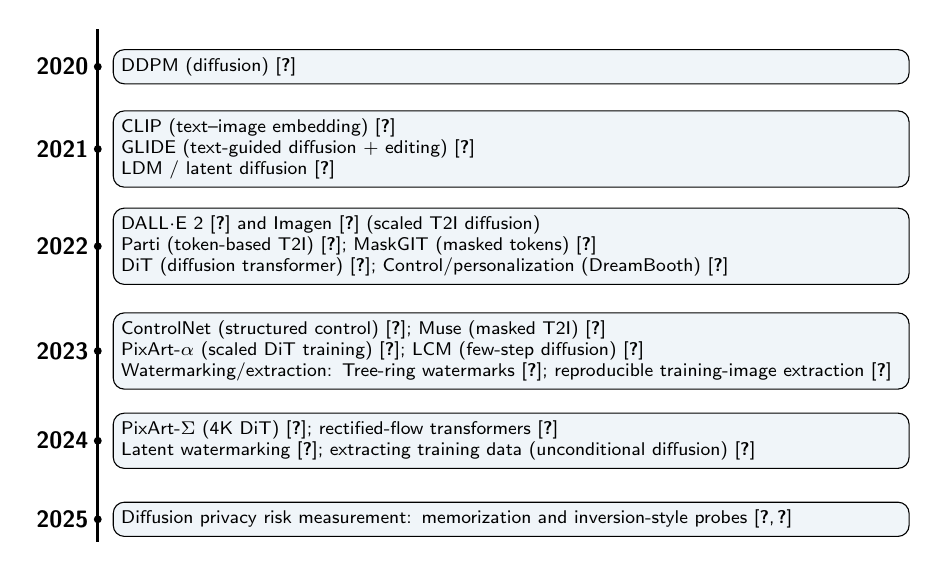
\begin{tikzpicture}[
        scale=0.95, transform shape,
        year/.style={font=\sffamily\bfseries\small, anchor=east},
        box/.style={rectangle, rounded corners, draw, fill=qubitblue!8, text=black,
            align=left, font=\sffamily\scriptsize, inner sep=3pt, text width=0.86\textwidth},
    ]
        \draw[very thick] (0,0.5) -- (0,-6.35);

        \node[year] (y2020) at (0,0) {2020};
        \node[box, anchor=west] at (0.2,0) {DDPM (diffusion) \cite{ho2020ddpm}};
        \fill (0,0) circle (1.5pt);

        \node[year] (y2021) at (0,-1.1) {2021};
        \node[box, anchor=west] at (0.2,-1.1) {CLIP (text--image embedding) \cite{radford2021clip}\\
        GLIDE (text-guided diffusion + editing) \cite{nichol2021glide}\\
        LDM / latent diffusion \cite{rombach2022ldm}};
        \fill (0,-1.1) circle (1.5pt);

        \node[year] (y2022) at (0,-2.4) {2022};
        \node[box, anchor=west] at (0.2,-2.4) {DALL\ensuremath{\cdot}E~2 \cite{ramesh2022dalle2} and Imagen \cite{saharia2022imagen} (scaled T2I diffusion)\\
        Parti (token-based T2I) \cite{yu2022parti}; MaskGIT (masked tokens) \cite{chang2022maskgit}\\
        DiT (diffusion transformer) \cite{peebles2022dit}; Control/personalization (DreamBooth) \cite{ruiz2022dreambooth}};
        \fill (0,-2.4) circle (1.5pt);

        \node[year] (y2023) at (0,-3.8) {2023};
        \node[box, anchor=west] at (0.2,-3.8) {ControlNet (structured control) \cite{zhang2023controlnet}; Muse (masked T2I) \cite{chang2023muse}\\
        PixArt-$\alpha$ (scaled DiT training) \cite{chen2023pixartalpha}; LCM (few-step diffusion) \cite{luo2023lcm}\\
        Watermarking/extraction: Tree-ring watermarks \cite{wen2023treering}; reproducible training-image extraction \cite{webster2023reproextraction}};
        \fill (0,-3.8) circle (1.5pt);

        \node[year] (y2024) at (0,-5.0) {2024};
        \node[box, anchor=west] at (0.2,-5.0) {PixArt-$\Sigma$ (4K DiT) \cite{chen2024pixartsigma}; rectified-flow transformers \cite{esser2024rectifiedflow}\\
        Latent watermarking \cite{meng2024latentwatermark}; extracting training data (unconditional diffusion) \cite{chen2024extractingunconditional}};
        \fill (0,-5.0) circle (1.5pt);

        \node[year] (y2025) at (0,-6.05) {2025};
        \node[box, anchor=west] at (0.2,-6.05) {Diffusion privacy risk measurement: memorization and inversion-style probes \cite{gu2025memorizationdiffusion,ma2025inversionmemorization}};
        \fill (0,-6.05) circle (1.5pt);
    \end{tikzpicture}
    \caption{Annotated timeline of representative research milestones in modern text-to-image generation (2020--2025). Entries are selected for illustrative coverage rather than completeness.}
    \label{fig:timeline}
\end{figure*}

% Tab 1: frontier comparison (two-column)
\begin{table*}[t]
    \centering
    \small
    \setlength{\tabcolsep}{4pt}
    \renewcommand{\arraystretch}{1.15}
    \caption{Frontier model comparison (illustrative; cite primary sources per row). Representative diffusion and token-based systems include LDM \cite{rombach2022ldm}, Imagen \cite{saharia2022imagen}, DALL\ensuremath{\cdot}E~2 \cite{ramesh2022dalle2}, DiT \cite{peebles2022dit}, PixArt-$\Sigma$ \cite{chen2024pixartsigma}, and Muse \cite{chang2023muse}.}
    \label{tab:frontier-models}
    \begin{tabular}{p{0.22\textwidth} p{0.22\textwidth} p{0.12\textwidth} p{0.36\textwidth}}
        \toprule
        \textbf{System} & \textbf{Backbone} & \textbf{Resolution} & \textbf{Openness} \\
        \midrule
        LDM / Stable Diffusion \cite{rombach2022ldm} & U-Net (latent diffusion) & High (latent) & Open weights (varies) \\
        Imagen \cite{saharia2022imagen} & U-Net diffusion & High & Closed weights/data \\
        DALL\ensuremath{\cdot}E~2 \cite{ramesh2022dalle2} & Diffusion + CLIP latents & High & Closed weights/data \\
        DiT \cite{peebles2022dit} & Transformer diffusion & High & Research code/paper \\
        PixArt-$\Sigma$ \cite{chen2024pixartsigma} & Diffusion transformer & 4{K} & Research code/paper \\
        Muse \cite{chang2023muse} & Masked token transformer & High & Closed weights/data \\
        \bottomrule
    \end{tabular}
\end{table*}

%%%%%%%%%%%%%%%%%%%%%%%%%%%%%%%%%%%%%%%%%
% EVALUATION
%%%%%%%%%%%%%%%%%%%%%%%%%%%%%%%%%%%%%%%%%
\section{Evaluation, Benchmarks, and Failure Modes}
\subsection{Metrics and Protocols}
Evaluating generative image models requires measuring multiple axes: sample fidelity, diversity, and alignment to conditioning
signals (e.g., text). For unconditional image synthesis, Inception Score (IS) and Fr\'echet Inception Distance (FID) are widely
used to quantify realism and distributional match, but they depend on feature extractors and can fail to reflect prompt
faithfulness in conditional generation \cite{salimans2016improvedgan,heusel2017fid}. Precision--recall-style metrics attempt to
separate fidelity and coverage, making tradeoffs more explicit \cite{kynkaanniemi2019pr}.

For text-to-image, embedding-based alignment metrics such as CLIPScore approximate prompt adherence by measuring similarity in a
joint image--text embedding space \cite{radford2021clip,hessel2021clipscore}. However, purely embedding-based metrics may miss
composition errors, hallucinated text, or safety violations, motivating mixed protocols that combine automatic scores with human
preferences and targeted test suites \cite{ramesh2022dalle2,saharia2022imagen,yu2022parti}.

Table~\ref{tab:eval-metrics} summarizes common metrics and their limitations in conditional generation settings.

% Tab 2 (placeholder): metrics/benchmarks
\begin{table}[t]
    \centering
    \caption{Common evaluation metrics and what they capture/miss in text-to-image settings. FID and IS quantify realism and distributional match \cite{heusel2017fid,salimans2016improvedgan}, precision/recall decomposes fidelity vs coverage \cite{kynkaanniemi2019pr}, and CLIPScore approximates prompt adherence \cite{hessel2021clipscore,radford2021clip}.}
    \label{tab:eval-metrics}
    \footnotesize
    \setlength{\tabcolsep}{4pt}
    \begin{tabular}{p{0.28\columnwidth} p{0.30\columnwidth} p{0.32\columnwidth}}
        \toprule
        \textbf{Metric} & \textbf{Captures} & \textbf{Misses} \\
        \midrule
        IS \cite{salimans2016improvedgan} & Classifier-based proxy for realism/diversity & Domain mismatch; weak for text alignment and composition \\
        FID \cite{heusel2017fid} & Feature-space distance to real images & Prompt adherence; semantic errors; feature/domain sensitivity \\
        Precision/Recall \cite{kynkaanniemi2019pr} & Separates fidelity vs coverage/diversity & Depends on feature space/thresholds; conditional alignment \\
        CLIPScore \cite{hessel2021clipscore,radford2021clip} & Text--image embedding similarity & Image realism; spatial correctness; safety violations \\
        \bottomrule
    \end{tabular}
\end{table}

\subsection{Failure Modes}
Common failure modes include prompt sensitivity (small prompt edits change outputs disproportionately), compositional errors
(incorrect attribute binding), and mode collapse or lack of diversity under strong guidance \cite{ho2022cfg,hessel2021clipscore}.
Editing and control introduce additional failure cases such as ``collateral edits'' and poor spatial adherence when the control
signal conflicts with the learned prior \cite{zhang2023controlnet,hertz2022prompttoprompt,brooks2022instructpix2pix}.

Because these failures often depend on the prompt distribution and the chosen guidance/sampler settings, reproducible evaluation
should document prompts, sampling parameters (steps, guidance scale), and any post-generation filtering \cite{lu2022dpmsolver,karras2022edm,ramesh2022dalle2}.

%%%%%%%%%%%%%%%%%%%%%%%%%%%%%%%%%%%%%%%%%
% SAFETY / PROVENANCE / OPEN PROBLEMS
%%%%%%%%%%%%%%%%%%%%%%%%%%%%%%%%%%%%%%%%%
\section{Safety, Provenance, and Open Problems}
\subsection{Safety, Misuse, and Governance}
Modern generative image systems raise safety issues spanning misuse (e.g., deception), privacy, and intellectual property.
From a data perspective, large-scale web datasets enable capability but also import biases and copyrighted or private content
into the training distribution, complicating downstream governance \cite{schuhmann2022laion5b,lin2014coco}. Many deployed
systems add layered mitigations (prompt and image filters, refusal policies, post-generation moderation), which can reduce
harmful outputs but also makes evaluation less transparent \cite{ramesh2022dalle2}.

Privacy risks have been studied through memorization and membership inference: attackers may test whether a training image
or concept was included in a model's training set, or attempt to recover training examples. Empirical work finds diffusion
models can be vulnerable to membership inference and that realistic threat models matter for measured risk
\cite{duan2023diffusionmembership,dubinski2023realisticmia}. Relatedly, multiple lines of work examine memorization behavior
in diffusion models and propose measurements and mitigations \cite{gu2025memorizationdiffusion,ma2025inversionmemorization}.

Data extraction results further show that, under some conditions, training images can be recovered from diffusion models,
highlighting a tension between scale, fidelity, and privacy \cite{webster2023reproextraction,chen2024extractingunconditional}.
These findings motivate cautious claims about ``generalization'' and suggest that SOTA reviews should treat privacy, data
curation, and filtering as first-class design choices rather than afterthoughts.

\subsection{Provenance and Watermarking}
Provenance mechanisms aim to help platforms and users identify AI-generated images or attribute outputs to a specific model.
One family of approaches embeds \emph{watermarks} by modifying the generation process so that outputs contain a detectable
signal while remaining visually indistinguishable. Tree-ring watermarks propose robust, invisible fingerprints tailored to
diffusion sampling \cite{wen2023treering}. Other methods watermark either the diffusion process itself or the latent space of
latent diffusion models, trading off robustness, detectability, and impact on image quality \cite{liu2023watermarkdiffusion,meng2024latentwatermark,peng2023watermarkdiffusionprocess}.

Watermarking is not a silver bullet: threat models include benign transformations (cropping, compression) and adaptive
attackers who attempt to remove or spoof watermarks. As a result, provenance systems are best viewed as components in a
broader pipeline (metadata standards, platform policies, and audit trails), with careful reporting of false-positive and
false-negative rates under realistic transformations \cite{wen2023treering,meng2024latentwatermark}.

\subsection{Open Problems and Recommendations}
We close with open problems that cut across model families:
(i) \emph{Evaluation}: develop prompt suites and metrics that better capture compositional correctness, text rendering,
and controllability, rather than optimizing toward a narrow set of proxy scores \cite{hessel2021clipscore,heusel2017fid}.
(ii) \emph{Efficiency}: push few-step generation without sacrificing diversity or introducing new artifacts, building on
solver and consistency ideas \cite{lu2022dpmsolver,song2023consistency}.
(iii) \emph{Control}: improve reliable spatial and semantic control without brittle prompt engineering, integrating adapters
and editing methods into coherent workflows \cite{zhang2023controlnet,brooks2022instructpix2pix}.
(iv) \emph{Safety and provenance}: quantify privacy risk and watermark robustness under realistic attackers, and standardize
disclosure practices for training data and filtering \cite{dubinski2023realisticmia,wen2023treering,webster2023reproextraction}.

For reproducible science, we recommend that papers report (a) prompt sets and sampling parameters, (b) the training data
mixture at a high level (or a data statement when full disclosure is impossible), and (c) evaluations that include both
automatic metrics and human or task-based protocols \cite{ramesh2022dalle2,saharia2022imagen}.

\section{Conclusion}
Modern generative image modeling is increasingly defined by scalable conditional generation: diffusion objectives and their
solver/distillation variants dominate many text-to-image settings, while token-based transformers remain competitive and offer
distinct efficiency tradeoffs \cite{ho2020ddpm,lu2022dpmsolver,chang2023muse}. The emergence of transformer backbones for
diffusion, alongside improved data and training recipes, has enabled rapid progress in photorealism and resolution
\cite{peebles2022dit,chen2024pixartsigma,esser2024rectifiedflow}.

At the same time, practical deployment depends on controllability, editing, and trustworthy evaluation. Adapter-based controls
and instruction editing provide powerful interfaces but expose new failure modes, and evaluation remains challenged by the
multi-objective nature of ``quality'' and the limitations of automatic metrics \cite{zhang2023controlnet,brooks2022instructpix2pix,hessel2021clipscore}.
Finally, safety and provenance are not optional: evidence on memorization, extraction, and watermark robustness shows that
responsible SOTA systems require end-to-end design that spans data, models, and governance \cite{webster2023reproextraction,wen2023treering,duan2023diffusionmembership}.

%%%%%%%%%%%%%%%%%%%%%%%%%%%%%%%%%%%%%%%%%
% BIBLIOGRAPHY
%%%%%%%%%%%%%%%%%%%%%%%%%%%%%%%%%%%%%%%%%
\clearpage
\bibliographystyle{ieeetr}  
\bibliography{ref} % References are in ref.bib

\end{document} 
